\documentclass[a4paper]{article}

\usepackage[utf8]{inputenc}
\usepackage[T1]{fontenc}
\usepackage{textcomp}
\usepackage[dutch]{babel}
\usepackage{amsmath, amssymb}
\usepackage{code}
\usepackage{pythonhighlight}

% figure support
\usepackage{import}
\usepackage{xifthen}
\pdfminorversion=7
\usepackage{pdfpages}
\usepackage{transparent}
\usepackage{graphicx}
\pdfsuppresswarningpagegroup=1
\graphicspath{{./img/}}

\begin{document}
   \section{Path planning} 
   \begin{itemize}
       \item Computing a route from starting point to a goal point
       \item assumptions
           \begin{itemize}
               \item where you are and where u need to go and map of environment(perception)
               \item behaviour of robot for command (math model)
               \item obstacles and open space where robot can move
           \end{itemize}
       \item Find the set of commands required to move the robot to the desired position - path planning
   \end{itemize}
   \section{Real time}
   \begin{itemize}
       \item something the happens without or negligible delay
       \item in robotics,procces with 10 hz or higher is considered as realtime
   \end{itemize}
   \section{Map representation}
   \begin{itemize}
       \item simplest map is a matrix of 0s and 1s
       \item continous map - represented as mathematical function (X>0 or X<5,Y>0 or Y6)
   \end{itemize}
   \section{path representation}
   \begin{itemize}
       \item series of interminent co-ordinates
       \item entire vector field which gives a direction and magnitude 
           \begin{itemize}
               \item \textbf{vector field} is a function where you give x and y and it gives direction and magnitude to move in
           \end{itemize}
   \end{itemize}
\section{list of algorithms}
\begin{itemize}
    \item Artificial potential fields
    \item Breadth first search 
    \item A* 
    \item RRT and RRT*
\end{itemize}
\subsection{Aritificial potential field}
\begin{itemize}
    \item $
        U(x,y) = distance\_from\_goal(x,y)  + \sum 1/distance\_from\_ith\_obstacle(x,y)
        $ 
    \begin{figure}[htpb]
                          \centering
                          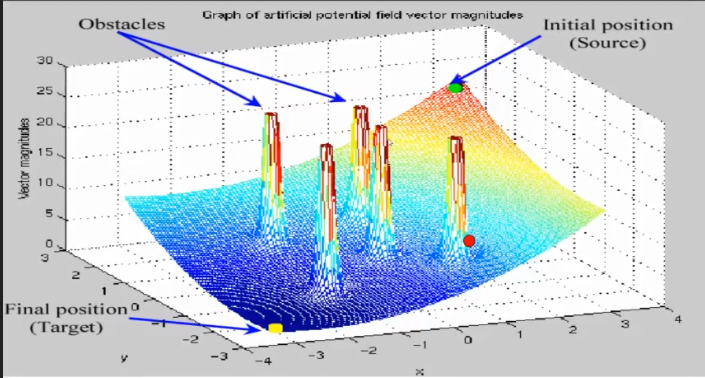
\includegraphics[width=0.8\textwidth]{field_vector_graph.png}
                          \caption{}
                          \label{fig:}
                      \end{figure}
    \item Find the gradient and move along negative direction
\end{itemize}
\end{document}
